% Gabarit pandoc des corrigés publiés (brut et guidé). Contenu sans marque ni nom de site.
% Compilation : lualatex (latexmk -lualatex).
% Le Markdown reste la source unique : ne pas éditer ce fichier .tex à la main.
\documentclass[11pt,a4paper]{article}

% --- Moteur, polices (Latin Modern) et langue ---------------------------------
\usepackage{iftex}
\ifLuaTeX\else\errmessage{Ce document se compile avec lualatex}\fi
\usepackage{amsmath,amssymb,mathtools}
\usepackage{fontspec}
% mathrm=sym : \mathrm prend ses glyphes dans la police mathématique (ℓ, μ, Ω), comme KaTeX.
\usepackage[math-style=TeX,bold-style=TeX,mathrm=sym]{unicode-math}
% Repli pour les glyphes absents de Latin Modern (indices et exposants Unicode,
% flèches, filets des schémas en texte, symboles) : DejaVu, puis Latin Modern Math
% (ℓ, lettres mathématiques Unicode des légendes).
\directlua{
  luaotfload.add_fallback("repliTexte", {"DejaVuSerif:mode=harf;", "DejaVuSans:mode=harf;", "file:latinmodern-math.otf:mode=harf;"})
  luaotfload.add_fallback("repliMono", {"DejaVuSansMono:mode=harf;", "DejaVuSans:mode=harf;", "file:latinmodern-math.otf:mode=harf;"})
}
\setmainfont{Latin Modern Roman}[RawFeature={fallback=repliTexte}]
\setsansfont{Latin Modern Sans}[RawFeature={fallback=repliTexte}]
\setmonofont{Latin Modern Mono}[RawFeature={fallback=repliMono}]
\setmathfont{Latin Modern Math}
\usepackage[french]{babel}
\frenchsetup{SmallCapsFigTabCaptions=false}

% --- Mise en page --------------------------------------------------------------
\usepackage[a4paper,margin=2.2cm,headheight=14pt,footskip=1.2cm]{geometry}
\usepackage{microtype}
\setlength{\emergencystretch}{4em}
\tolerance=1500
\setlength{\parindent}{0pt}
\setlength{\parskip}{0.55\baselineskip plus 2pt minus 1pt}
\usepackage{xcolor}
% Gris nommés : babel-french rend « ! » actif dans le document.
\definecolor{gris2}{gray}{0.98}
\definecolor{gris3}{gray}{0.97}
\definecolor{gris5}{gray}{0.95}
\definecolor{gris35}{gray}{0.65}
\definecolor{gris40}{gray}{0.60}
\definecolor{gris45}{gray}{0.55}
\definecolor{gris50}{gray}{0.50}
\definecolor{gris55}{gray}{0.45}
\definecolor{gris60}{gray}{0.40}
\definecolor{gris65}{gray}{0.35}
\definecolor{gris70}{gray}{0.30}
\definecolor{gris80}{gray}{0.20}
\definecolor{gris85}{gray}{0.15}
\usepackage{graphicx}
\usepackage{float}
\usepackage{caption}
\captionsetup{font=small,labelformat=empty,justification=centering}
\usepackage{booktabs,longtable,array,multirow,calc}
\usepackage{siunitx}
\sisetup{locale=FR}
\usepackage[version=4]{mhchem}
\usepackage{listings}
\usepackage{fancyhdr}
\usepackage{lastpage}
\usepackage[most]{tcolorbox}
\usepackage{enumitem}
\setlist{nosep,leftmargin=*,topsep=2pt}
\usepackage[hidelinks,unicode]{hyperref}
\usepackage{bookmark}
\hypersetup{pdftitle={Centrale-Supélec MP-MPI — Mathématiques 2 2026},pdfauthor={Rédigé par IA},pdfcreator={LaTeX},pdfsubject={Corrigé guidé}}
\usepackage{xurl}

% --- Pandoc : listes, tableaux, figures ----------------------------------------
\providecommand{\passthrough}[1]{#1}
\providecommand{\tightlist}{\setlength{\itemsep}{0pt}\setlength{\parskip}{0pt}}

\makeatletter
\def\maxwidth{\ifdim\Gin@nat@width>\linewidth\linewidth\else\Gin@nat@width\fi}
\def\maxheight{\ifdim\Gin@nat@height>0.55\textheight 0.55\textheight\else\Gin@nat@height\fi}
\makeatother
\setkeys{Gin}{width=\maxwidth,height=\maxheight,keepaspectratio}
\setcounter{secnumdepth}{-\maxdimen}
\providecommand{\pandocbounded}[1]{#1}
\usepackage{longtable,booktabs,array}

% --- Code (listings) -----------------------------------------------------------
\lstset{
  basicstyle=\ttfamily\small,
  columns=fullflexible,
  keepspaces=true,
  breaklines=true,
  breakatwhitespace=false,
  postbreak=\mbox{\textcolor{gris50}{$\hookrightarrow$}\space},
  frame=single,
  rulecolor=\color{gris35},
  framesep=4pt,
  xleftmargin=5pt,xrightmargin=5pt,
  backgroundcolor=\color{gris3},
  keywordstyle=\bfseries,
  commentstyle=\color{gris65},
  stringstyle=\color{gris80},
  showstringspaces=false,
  tabsize=4,
  extendedchars=true,
  aboveskip=6pt,belowskip=6pt,
}

% --- Macros des corrigés (KaTeX ↔ LaTeX) ---------------------------------------
% Les corrigés sont écrits pour KaTeX : on définit ici ce que KaTeX connaît et
% que LaTeX n'a pas, sans jamais retoucher le Markdown.
\providecommand{\R}{\mathbb{R}}
\providecommand{\N}{\mathbb{N}}
\providecommand{\Z}{\mathbb{Z}}
\providecommand{\Q}{\mathbb{Q}}
\providecommand{\C}{\mathbb{C}}
\providecommand{\dd}{\mathrm{d}}
\providecommand{\llbracket}{\lBrack}
\providecommand{\rrbracket}{\rBrack}
\providecommand{\lBrace}{\lbrace}
\providecommand{\rBrace}{\rbrace}
\providecommand{\Box}{\square}
\providecommand{\Diamond}{\lozenge}
\providecommand{\varnothing}{\emptyset}
\providecommand{\argmax}{\operatorname*{arg\,max}}
\providecommand{\argmin}{\operatorname*{arg\,min}}
\renewcommand{\leq}{\leqslant}
\renewcommand{\geq}{\geqslant}

% Équation hors texte : réduite à la largeur de la ligne si elle déborde.
\newsavebox{\boiteequation}
\newcommand{\equationajustee}[1]{%
  \sbox{\boiteequation}{$\displaystyle #1$}%
  \ifdim\wd\boiteequation>\linewidth
    \[\resizebox{\linewidth}{!}{\usebox{\boiteequation}}\]%
  \else
    \[#1\]%
  \fi}

% --- Encadrés pédagogiques (sobres, lisibles en noir et blanc) -----------------
\tcbset{
  encadre/.style={
    enhanced,breakable,sharp corners,
    colback=white,colframe=gris55,
    boxrule=0.4pt,leftrule=2.2pt,
    left=6pt,right=6pt,top=3pt,bottom=3pt,
    before skip=6pt,after skip=6pt,
    fonttitle=\bfseries\small,coltitle=black,
    attach title to upper,after title={\quad},
    parbox=false,
  }
}
\newtcolorbox{indication}[1]{encadre,colframe=gris45,colback=gris2,title={Indication~#1}}
\newtcolorbox{methode}{encadre,colframe=gris70,title={Méthode}}
\newtcolorbox{piege}{encadre,colframe=gris85,boxrule=0.8pt,leftrule=2.2pt,title={Piège}}
\newtcolorbox{jury}{encadre,colframe=gris60,colback=gris5,title={Jury}}
\newtcolorbox{encadrenote}{encadre,colframe=gris40}

% --- Titres de section ---------------------------------------------------------
\usepackage{titlesec}
\titleformat{\section}{\Large\bfseries}{}{0pt}{}
\titleformat{\subsection}{\large\bfseries}{}{0pt}{}
\titleformat{\subsubsection}{\normalsize\bfseries}{}{0pt}{}
\titlespacing*{\section}{0pt}{14pt plus 4pt minus 2pt}{6pt}
\titlespacing*{\subsection}{0pt}{10pt plus 3pt minus 2pt}{4pt}
\titlespacing*{\subsubsection}{0pt}{8pt plus 2pt minus 2pt}{2pt}

% --- En-tête et pied de page ---------------------------------------------------
\pagestyle{fancy}
\fancyhf{}
\fancyhead[L]{\small\textsc{Corrigé guidé} · Centrale-Supélec MP-MPI}
\fancyhead[R]{\small Maths 2 2026}
\fancyfoot[L]{\footnotesize Corrigé rédigé par IA, non officiel}
\fancyfoot[R]{\footnotesize \thepage\,/\,\pageref*{LastPage}}
\renewcommand{\headrulewidth}{0.4pt}
\renewcommand{\footrulewidth}{0pt}
\fancypagestyle{plain}{\fancyhf{}\fancyfoot[R]{\footnotesize \thepage\,/\,\pageref*{LastPage}}\fancyfoot[L]{\footnotesize Corrigé rédigé par IA, non officiel}\renewcommand{\headrulewidth}{0pt}}

\begin{document}
\thispagestyle{plain}
\begin{center}
  {\small\scshape Corrigé guidé}\par\smallskip
  {\LARGE\bfseries Centrale-Supélec MP-MPI — Mathématiques 2 2026\par}\medskip
  {\large Centrale-Supélec · MP-MPI · Maths 2 · 2026\par}
\end{center}
\vspace{2pt}\hrule\vspace{8pt}

\emph{Corrigé rédigé par IA, non officiel. Signalez toute erreur.}

\hypertarget{pruxe9sentation-du-sujet}{%
\section{Présentation du sujet}\label{pruxe9sentation-du-sujet}}

\textbf{Thème.} Le sujet construit une \emph{condition suffisante} pour que la fonction \(\zeta\) de Riemann ne s'annule pas dans le demi-plan \(\operatorname{Re}(s)>\frac12\) (forme de l'hypothèse de Riemann). Cette condition est géométrique : si la distance \(d_n\), dans un espace de fonctions de carré intégrable sur \(]0,1]\), de la fonction constante \(\mathbf 1\) au sous-espace engendré par \(f_2,\dots,f_n\), où
\equationajustee{f_k(t)=\frac1k\Bigl\lfloor\frac1t\Bigr\rfloor-\Bigl\lfloor\frac1{kt}\Bigr\rfloor,}
tend vers \(0\), alors \(\zeta\) n'a pas de zéro de partie réelle \(>\frac12\). Le résultat appartient à la famille des critères dits de Nyman-Beurling ; le sujet n'en démontre qu'un sens et ne prétend évidemment pas établir que \(d_n\to0\).

\textbf{Découpage.}

\begin{longtable}[]{@{}
  >{\raggedright\arraybackslash}p{(\columnwidth - 6\tabcolsep) * \real{0.1169}}
  >{\raggedright\arraybackslash}p{(\columnwidth - 6\tabcolsep) * \real{0.1432}}
  >{\raggedright\arraybackslash}p{(\columnwidth - 6\tabcolsep) * \real{0.3758}}
  >{\raggedright\arraybackslash}p{(\columnwidth - 6\tabcolsep) * \real{0.3341}}@{}}
\toprule\noalign{}
\begin{minipage}[b]{\linewidth}\raggedright
Partie
\end{minipage} & \begin{minipage}[b]{\linewidth}\raggedright
Questions
\end{minipage} & \begin{minipage}[b]{\linewidth}\raggedright
Contenu
\end{minipage} & \begin{minipage}[b]{\linewidth}\raggedright
Outils
\end{minipage} \\
\midrule\noalign{}
\endhead
\bottomrule\noalign{}
\endlastfoot
A-I & Q1--Q3 & \(\zeta\) sur \(]1,+\infty[\) : convergence normale, continuité, signe & séries de fonctions \\
A-II & Q4--Q10 & produit eulérien, non-annulation sur \(\operatorname{Re}(s)>1\) & familles sommables, séries numériques, logarithme \\
A-III & Q11 & \(\int_0^1|t^{s-1}|^2=\frac1{2\operatorname{Re}(s)-1}\) & intégrales de Riemann \\
A-IV & Q12--Q14 & disques \(\mathcal D_d\), intersection des \(\Delta_d\) & géométrie du plan complexe, étude de fonction \\
B-I & Q15--Q21 & valeurs et paliers des \(f_k\), transformée de Mellin & partie entière, intégrales généralisées \\
B-II & Q22--Q24 & prolongement \(\zeta(s)=\frac1{s-1}+G(s)\) & comparaison série-intégrale, accroissements finis \\
B-III & Q25--Q26 & \(\int_0^1f_k=\frac{\ln k}k\) & passage à la limite, développement limité \\
C-I & Q27--Q29 & l'espace \(L^2\) et la forme \((f|g)=\int fg\) & intégrabilité, comparaison \\
C-II & Q30--Q33 & liberté de \((f_k)\), produit scalaire sur \(F\) & algèbre linéaire, partie entière \\
C-III & Q34--Q36 & Gram-Schmidt, distance \(d_n\) & espaces préhilbertiens \\
D & Q37--Q38 & Cauchy-Schwarz et conclusion & synthèse \\
\end{longtable}

\textbf{Notions du programme mobilisées.} Convergence normale et continuité des séries de fonctions ; familles sommables (produit, sommation par paquets, réindexation) ; séries à termes positifs ; intégrales généralisées et comparaison ; théorème de convergence dominée (ou majoration directe) ; espaces préhilbertiens, Gram-Schmidt, projection orthogonale, Pythagore ; nombres complexes.

\textbf{Difficulté et longueur.} Sujet long (38 questions en 4 heures, soit un peu plus de 6 minutes par question) mais très progressif : la plupart des questions sont des applications directes du cours, et la difficulté se concentre sur quelques points (Q7, Q16, Q20--Q21, Q26, Q32--Q34, Q38). Les parties sont largement indépendantes : A-III et A-IV ne dépendent de rien, B-II ne dépend pas de B-I, et la partie D peut se traiter en admettant Q11, Q21 et Q35.

\textbf{Questions abordables à ne pas laisser passer.} Q1--Q5, Q11, Q12--Q14, Q15, Q17, Q22--Q23, Q27--Q30, Q35--Q37. Elles représentent près de la moitié du sujet.

\textbf{Gestion du temps.} Viser environ 1 h pour la partie A, 1 h 15 pour la partie B, 1 h 15 pour la partie C et 30 min pour la partie D. Ne pas s'enliser dans les questions de rédaction délicate (Q7, Q20) : leurs résultats sont donnés et utilisables pour la suite.

\hypertarget{partie-a-questions-pruxe9liminaires}{%
\section{Partie A --- Questions préliminaires}\label{partie-a-questions-pruxe9liminaires}}

Cette partie rassemble les propriétés de base de \(\zeta\) sur \(]1,+\infty[\) puis sur \(\operatorname{Re}(s)>1\), où l'on montre la non-annulation grâce au produit eulérien. Elle prépare aussi deux outils autonomes : l'intégrale de Q11 et la famille de disques de Q12--Q14.

\hypertarget{a.i-la-fonction-zeta-sur-lintervalle-1infty}{%
\subsection{\texorpdfstring{A.I --- La fonction \(\zeta\) sur l'intervalle \(]1,+\infty[\)}{A.I --- La fonction \textbackslash zeta sur l'intervalle {]}1,+\textbackslash infty{[}}}\label{a.i-la-fonction-zeta-sur-lintervalle-1infty}}

\hypertarget{question-1}{%
\subsection{Question 1}\label{question-1}}

\begin{indication}{1}

Calculer la norme infinie de \(u_k\) sur \(]1,+\infty[\) : où le maximum de \(s\mapsto k^{-s}\) est-il « approché » ?

\end{indication}

\begin{indication}{2}

La norme obtenue est une borne supérieure non atteinte ; reconnaître la série numérique associée.

\end{indication}

\hypertarget{solution}{%
\subsubsection{Solution}\label{solution}}

Pour \(k\geqslant1\), \(s\mapsto k^{-s}=e^{-s\ln k}\) est décroissante (\(\ln k\geqslant0\)), donc
\equationajustee{\begin{aligned}\|u_k\|_{\infty,]1,+\infty[}&=\sup_{s>1}k^{-s}\\&=\lim_{s\to1^+}k^{-s}\\&=\frac1k.\end{aligned}}
La série harmonique diverge : \textbf{la série \(\sum u_k\) ne converge pas normalement sur \(]1,+\infty[\).}

En revanche, sur \([a,+\infty[\) avec \(a>1\), \(\|u_k\|_\infty=k^{-a}\) et \(\sum k^{-a}\) converge : la convergence y est normale.

\begin{piege}

Majorer \(k^{-s}\) par \(k^{-s_0}\) pour un \(s_0>1\) fixé ne donne pas une majoration valable pour \emph{tous} les \(s>1\). La convergence normale est une propriété uniforme sur l'intervalle entier.

\end{piege}

\hypertarget{question-2}{%
\subsection{Question 2}\label{question-2}}

\begin{indication}{1}

La continuité est une propriété locale : il suffit d'avoir convergence uniforme au voisinage de chaque point.

\end{indication}

\begin{indication}{2}

Autour de \(s_0>1\), choisir un intervalle \([a,+\infty[\) avec \(1<a<s_0\) et utiliser la fin de Q1.

\end{indication}

\hypertarget{solution-1}{%
\subsubsection{Solution}\label{solution-1}}

Soit \(s_0>1\) et \(a=\frac{1+s_0}2\in\,]1,s_0[\). Les \(u_k\) sont continues et \(\sum u_k\) converge normalement, donc uniformément, sur \([a,+\infty[\).

Par le théorème de continuité de la somme d'une série de fonctions, \(\zeta\) est continue sur \([a,+\infty[\), donc en \(s_0\) (point intérieur). Comme \(s_0\) est quelconque, \textbf{\(\zeta\) est continue sur \(]1,+\infty[\).}

\begin{methode}

Quand la convergence normale échoue sur l'intervalle entier à cause d'une borne, on la cherche sur tout segment ou sur tout \([a,+\infty[\) intérieur, puis on conclut par le caractère local de la continuité.

\end{methode}

\hypertarget{question-3}{%
\subsection{Question 3}\label{question-3}}

\begin{indication}{1}

Une somme de termes strictement positifs majore chacune de ses sommes partielles.

\end{indication}

\hypertarget{solution-2}{%
\subsubsection{Solution}\label{solution-2}}

Pour \(s>1\), les termes \(k^{-s}\) sont strictement positifs, donc \(\zeta(s)\geqslant1^{-s}=1\) :
\equationajustee{\boxed{\zeta(s)\geqslant1>0.}}
\textbf{\(\zeta\) ne s'annule pas sur \(]1,+\infty[\) et y est strictement positive.}

\hypertarget{a.ii-cas-de-la-variable-complexe}{%
\subsection{A.II --- Cas de la variable complexe}\label{a.ii-cas-de-la-variable-complexe}}

\hypertarget{question-4}{%
\subsection{Question 4}\label{question-4}}

\begin{indication}{1}

Revenir à la définition \(t^s=e^{s\ln t}\) et au module d'une exponentielle complexe.

\end{indication}

\hypertarget{solution-3}{%
\subsubsection{Solution}\label{solution-3}}

Avec \(s=x+iy\), \(s\ln t=x\ln t+iy\ln t\) et \(|e^z|=e^{\operatorname{Re}z}\), donc
\equationajustee{\boxed{|t^s|=t^{\operatorname{Re}(s)}}}
et \(\operatorname{Im}(s)\) n'intervient pas (le facteur \(e^{iy\ln t}\) est de module \(1\)).

\begin{piege}

Écrire \(|t^s|=t^{|s|}\) est une faute grave : seule la partie réelle compte. Ce résultat sera utilisé à chaque majoration de la suite.

\end{piege}

\hypertarget{question-5}{%
\subsection{Question 5}\label{question-5}}

\begin{indication}{1}

Calculer le module du terme général grâce à Q4 et reconnaître une série de référence.

\end{indication}

\hypertarget{solution-4}{%
\subsubsection{Solution}\label{solution-4}}

Par Q4, \(|k^{-s}|=k^{-x}\) avec \(x=\operatorname{Re}(s)>1\) : série de Riemann convergente. \textbf{La série \(\sum k^{-s}\) converge absolument}, donc converge dans \(\mathbb C\).

\hypertarget{question-6}{%
\subsection{Question 6}\label{question-6}}

\begin{indication}{1}

Écrire le terme général comme un produit de \(n\) facteurs, chacun ne dépendant que d'un \(m_i\).

\end{indication}

\begin{indication}{2}

Chaque facteur décrit une famille géométrique ; vérifier que sa raison est de module \(<1\), puis invoquer le théorème sur le produit de familles sommables.

\end{indication}

\hypertarget{solution-5}{%
\subsubsection{Solution}\label{solution-5}}

Pour \(a,b>0\), \((ab)^s=a^sb^s\) et \((p^m)^s=(p^s)^m\) (propriétés de l'exponentielle). Avec \(q_i=p_i^{-s}\),
\equationajustee{\frac1{(p_1^{m_1}\cdots p_n^{m_n})^s}=\prod_{i=1}^nq_i^{m_i}.}
Par Q4, \(|q_i|=p_i^{-x}\leqslant2^{-x}<1\), donc la famille \((q_i^m)_{m\in\mathbb N}\) est sommable, de somme \(\frac1{1-q_i}\). Le théorème du produit de familles sommables (cas de deux familles, puis récurrence sur \(n\)) donne la sommabilité de la famille produit indexée par \(\mathbb N^n\) et
\equationajustee{\boxed{S_n(s)=\prod_{i=1}^n\frac1{1-\frac1{p_i^s}}.}}

\begin{methode}

Une somme sur \(\mathbb N^n\) dont le terme général est un produit de fonctions de chaque indice se calcule comme produit de sommes, à condition d'avoir établi la sommabilité de chaque facteur.

\end{methode}

\hypertarget{question-7}{%
\subsection{Question 7}\label{question-7}}

\begin{indication}{1}

Le théorème fondamental de l'arithmétique fournit une bijection entre \(\mathbb N^n\) et \(\mathbb N_n\).

\end{indication}

\begin{indication}{2}

Pour la limite, majorer \(|\zeta(s)-S_n(s)|\) par une somme portant sur les entiers qui ne sont pas dans \(\mathbb N_n\), et remarquer que ces entiers sont tous grands.

\end{indication}

\hypertarget{solution-6}{%
\subsubsection{Solution}\label{solution-6}}

L'application \((m_1,\dots,m_n)\mapsto p_1^{m_1}\cdots p_n^{m_n}\) est une bijection de \(\mathbb N^n\) sur \(\mathbb N_n\) (existence et unicité de la décomposition en facteurs premiers). La somme d'une famille sommable ne dépendant pas de l'indexation,
\equationajustee{S_n(s)=\sum_{k\in\mathbb N_n}\frac1{k^s}.}
La famille \((k^{-s})_{k\geqslant1}\) est sommable (Q5) ; par sommation par paquets,
\equationajustee{|\zeta(s)-S_n(s)|=\Bigl|\sum_{k\in\mathbb N^*\setminus\mathbb N_n}k^{-s}\Bigr|\leqslant\sum_{k\in\mathbb N^*\setminus\mathbb N_n}k^{-x}.}
Tout entier \(k\leqslant p_n\) n'a que des facteurs premiers \(\leqslant p_n\), donc appartient à \(\mathbb N_n\). Par contraposée,
\equationajustee{|\zeta(s)-S_n(s)|\leqslant\sum_{k>p_n}\frac1{k^x}\xrightarrow[n\to+\infty]{}0}
(reste d'une série convergente, \(p_n\to+\infty\)). Donc
\equationajustee{\boxed{\lim_{n\to+\infty}S_n(s)=\zeta(s).}}

\begin{piege}

Le reste se coupe en \(p_n\), pas en \(n\). Et l'argument arithmétique « tout \(k\leqslant p_n\) est dans \(\mathbb N_n\) » est le cœur de la question : il doit être écrit.

\end{piege}

\hypertarget{question-8}{%
\subsection{Question 8}\label{question-8}}

\begin{indication}{1}

Prendre le logarithme de \(S_n(x)\) (produit fini) : on obtient la somme partielle d'une série à termes positifs.

\end{indication}

\begin{indication}{2}

Comparer ensuite \(-\ln(1-u)\) et \(u\) pour \(u\in[0,1[\).

\end{indication}

\hypertarget{solution-7}{%
\subsubsection{Solution}\label{solution-7}}

Pour \(x>1\) réel, \(S_n(x)>0\) et \(S_n(x)\to\zeta(x)\geqslant1\) (Q7, Q3), donc
\equationajustee{\ln S_n(x)=\sum_{i=1}^n-\ln(1-p_i^{-x})\xrightarrow[n\to+\infty]{}\ln\zeta(x).}
La série à termes positifs \(\sum_i-\ln(1-p_i^{-x})\) a des sommes partielles convergentes, donc converge.

L'étude de \(\psi(u)=-\ln(1-u)-u\) (\(\psi(0)=0\), \(\psi'(u)=\frac u{1-u}\geqslant0\)) donne \(0\leqslant u\leqslant-\ln(1-u)\) sur \([0,1[\). Par comparaison, \textbf{\(\sum_i p_i^{-x}\) converge.}

\begin{methode}

Pour étudier un produit, on passe au logarithme d'un produit \emph{fini}, puis on fait tendre \(n\) vers l'infini. Les inégalités \(u\leqslant-\ln(1-u)\) et \(\ln(1+u)\leqslant u\) se démontrent en une ligne par étude de fonction.

\end{methode}

\hypertarget{question-9}{%
\subsection{Question 9}\label{question-9}}

\begin{indication}{1}

Suivre l'énoncé : \(\ln a_n\) est la somme partielle d'une série de signe constant.

\end{indication}

\begin{indication}{2}

Majorer \(\ln(1+u)\) par \(u\) et utiliser Q8 ; la stricte positivité de la limite vient de ce que le logarithme converge vers un réel fini.

\end{indication}

\hypertarget{solution-8}{%
\subsubsection{Solution}\label{solution-8}}

On a \(\frac{p_i^x}{p_i^x+1}=\frac1{1+p_i^{-x}}\), donc
\equationajustee{\ln a_n=-\sum_{i=1}^n\ln(1+p_i^{-x}).}
Comme \(0\leqslant\ln(1+u)\leqslant u\) pour \(u\geqslant0\), Q8 et la comparaison donnent la convergence de \(\sum\ln(1+p_i^{-x})\), de somme \(L\geqslant0\).

Ainsi \(\ln a_n\to-L\) et
\equationajustee{\boxed{a_n\to e^{-L}>0.}}

\begin{piege}

La suite \((a_n)\) est décroissante et positive, donc convergente, mais cela ne dit rien du signe strict de la limite. C'est la convergence de \(\ln a_n\) vers un réel qui l'assure.

\end{piege}

\hypertarget{question-10}{%
\subsection{Question 10}\label{question-10}}

\begin{indication}{1}

Minorer \(|S_n(s)|\) facteur par facteur : il faut \emph{majorer} chaque \(|1-p_i^{-s}|\).

\end{indication}

\begin{indication}{2}

Passer ensuite à la limite avec Q7 et Q9.

\end{indication}

\hypertarget{solution-9}{%
\subsubsection{Solution}\label{solution-9}}

Comme \(|p_i^{-s}|=p_i^{-x}<1\), on a \(1-p_i^{-s}\neq0\) et
\equationajustee{|1-p_i^{-s}|\leqslant1+p_i^{-x}=\frac{p_i^x+1}{p_i^x}.}
En inversant et en multipliant :
\equationajustee{|S_n(s)|=\prod_{i=1}^n\frac1{|1-p_i^{-s}|}\geqslant a_n.}
Par passage à la limite (Q7, Q9), \(|\zeta(s)|\geqslant e^{-L}>0\). \textbf{Donc \(\zeta(s)\neq0\) pour \(\operatorname{Re}(s)>1\).}

\begin{piege}

C'est l'inégalité triangulaire \(|1-z|\leqslant1+|z|\) qui sert, pas \(|1-z|\geqslant1-|z|\). Penser aussi à justifier que les facteurs sont non nuls avant d'inverser.

\end{piege}

\hypertarget{a.iii-un-calcul-dintuxe9grale}{%
\subsection{A.III --- Un calcul d'intégrale}\label{a.iii-un-calcul-dintuxe9grale}}

\hypertarget{question-11}{%
\subsection{Question 11}\label{question-11}}

\begin{indication}{1}

Par Q4, le module de \(t^{2(s-1)}\) est une puissance réelle de \(t\) ; reconnaître une intégrale de Riemann en \(0\).

\end{indication}

\hypertarget{solution-10}{%
\subsubsection{Solution}\label{solution-10}}

Avec \(x=\operatorname{Re}(s)>\frac12\), Q4 donne
\equationajustee{|t^{2(s-1)}|=t^{2x-2}=t^{-(2-2x)},}
avec \(2-2x<1\) : intégrale de Riemann convergente en \(0\). Donc \(t\mapsto t^{2(s-1)}\) (continue sur \(]0,1]\)) est intégrable.

Comme \(|t^{s-1}|^2=t^{2x-2}\),
\equationajustee{\begin{aligned}\int_0^1|t^{s-1}|^2\,\mathrm dt&=\lim_{\varepsilon\to0^+}\Bigl[\frac{t^{2x-1}}{2x-1}\Bigr]_\varepsilon^1\\&=\boxed{\frac1{2\operatorname{Re}(s)-1}}.\end{aligned}}

\begin{methode}

Pour une puissance complexe, on intègre le module : \(|t^{\alpha}|=t^{\operatorname{Re}\alpha}\) ramène tout au critère de Riemann. C'est ici qu'apparaît la droite \(\operatorname{Re}(s)=\frac12\).

\end{methode}

\hypertarget{a.iv-une-uxe9tude-guxe9omuxe9trique}{%
\subsection{A.IV --- Une étude géométrique}\label{a.iv-une-uxe9tude-guxe9omuxe9trique}}

\hypertarget{question-12}{%
\subsection{Question 12}\label{question-12}}

\begin{indication}{1}

Écrire \(s=X+iY\) et diviser par \(d^2\).

\end{indication}

\begin{indication}{2}

Compléter le carré en \(X\) pour reconnaître l'équation d'un cercle.

\end{indication}

\hypertarget{solution-11}{%
\subsubsection{Solution}\label{solution-11}}

\equationajustee{\begin{aligned}s\in\Delta_d&\iff X^2+Y^2-\frac{2X}{d^2}+\frac1{d^2}\geqslant0\\&\iff\Bigl(X-\frac1{d^2}\Bigr)^2+Y^2\geqslant\frac{1-d^2}{d^4}.\end{aligned}}
Comme \(1-d^2>0\), \(\Delta_d\) est le complémentaire du \textbf{disque ouvert} \(\mathcal D_d\) de
\equationajustee{\boxed{\begin{aligned}{}&\text{centre }O_d=\frac1{d^2},\\&\text{rayon }R_d=\frac{\sqrt{1-d^2}}{d^2}.\end{aligned}}}

\begin{piege}

L'inégalité est large, donc le cercle appartient à \(\Delta_d\) et le disque retiré est ouvert.

\end{piege}

\hypertarget{question-13}{%
\subsection{Question 13}\label{question-13}}

\begin{indication}{1}

L'expression est indéterminée en \(0\) : multiplier par la quantité conjuguée.

\end{indication}

\begin{indication}{2}

Sous la forme obtenue, la monotonie se lit sans dériver.

\end{indication}

\hypertarget{solution-12}{%
\subsubsection{Solution}\label{solution-12}}

\equationajustee{\begin{aligned}g(d)&=\frac{1-\sqrt{1-d^2}}{d^2}\\&=\frac{1}{1+\sqrt{1-d^2}}.\end{aligned}}
La fonction \(d\mapsto\sqrt{1-d^2}\) est continue, strictement décroissante sur \(]0,1[\), de limites \(1\) en \(0^+\) et \(0\) en \(1^-\).

Donc \(g\) est continue, strictement croissante, de limites \(\frac12\) et \(1\), et par le théorème de la bijection
\equationajustee{\boxed{g(]0,1[)=\Bigl]\frac12,1\Bigr[.}}
Interprétation : \(g(d)=O_d-R_d\) est l'abscisse du point le plus à gauche de \(\mathcal D_d\).

\hypertarget{question-14}{%
\subsection{Question 14}\label{question-14}}

\begin{indication}{1}

Raisonner par double inclusion ; l'une des inclusions est immédiate selon le signe de \(2\operatorname{Re}(s)-1\).

\end{indication}

\begin{indication}{2}

Pour l'autre, faire tendre \(d\) vers \(0\) dans l'inégalité large.

\end{indication}

\hypertarget{solution-13}{%
\subsubsection{Solution}\label{solution-13}}

Si \(\operatorname{Re}(s)\leqslant\frac12\), alors \(2\operatorname{Re}(s)-1\leqslant0\leqslant d^2|s|^2\) : \(s\in\Delta_d\) pour tout \(d\).

Réciproquement, si \(2\operatorname{Re}(s)-1\leqslant d^2|s|^2\) pour tout \(d\in\,]0,1[\), le passage à la limite \(d\to0^+\) donne \(2\operatorname{Re}(s)-1\leqslant0\). Donc
\equationajustee{\boxed{\bigcap_{d\in]0,1[}\Delta_d=\Bigl\{s:\operatorname{Re}(s)\leqslant\frac12\Bigr\}.}}

\begin{figure}[H]
\centering
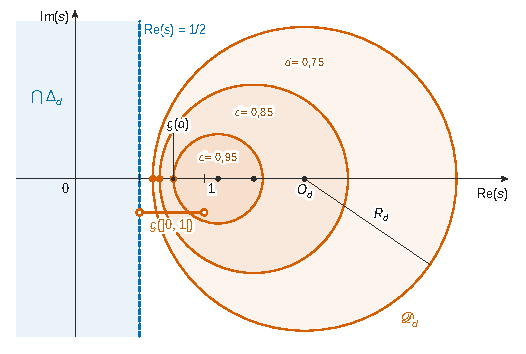
\includegraphics{figures/q14-disques-delta-d.pdf}
\caption*{Figure 1 --- disques 𝒟\_d pour d = 0,95 ; 0,85 ; 0,75, dont le bord
gauche g(d) est strictement entre 1/2 et 1 ; l'intersection des Δ\_d est
le demi-plan fermé Re(s) ⩽ 1/2 (Q12--Q14)}
\end{figure}

Quand \(d\to0^+\), centre et rayon tendent vers \(+\infty\) : la réunion des disques \(\mathcal D_d\) est le demi-plan ouvert \(\operatorname{Re}(s)>\frac12\).

\begin{piege}

On ne peut pas « prendre \(d=0\) », qui n'est pas dans \(]0,1[\) : on passe à la limite dans une inégalité large.

\end{piege}

\hypertarget{partie-b-uxe9tude-analytique}{%
\section{Partie B --- Étude analytique}\label{partie-b-uxe9tude-analytique}}

On étudie les fonctions \(f_k\) : leurs valeurs (Q15--Q17), leur structure en paliers (Q18), puis leur transformée de Mellin \(\int_0^1f_k(t)t^{s-1}\,\mathrm dt\), qui fait apparaître \(\zeta\) en facteur (Q19--Q21). On prolonge ensuite \(\zeta\) à \(\operatorname{Re}(s)>0\) et on en déduit \(\int_0^1f_k\).

\hypertarget{b.i-transformuxe9e-de-mellin-des-fonctions-f_k}{%
\subsection{\texorpdfstring{B.I --- Transformée de Mellin des fonctions \(f_k\)}{B.I --- Transformée de Mellin des fonctions f\_k}}\label{b.i-transformuxe9e-de-mellin-des-fonctions-f_k}}

\hypertarget{question-15}{%
\subsection{Question 15}\label{question-15}}

\begin{indication}{1}

En \(t=\frac1i\), la première partie entière est immédiate ; distinguer \(i<k\) et \(i=k\) pour la seconde.

\end{indication}

\hypertarget{solution-14}{%
\subsubsection{Solution}\label{solution-14}}

\(\lfloor\frac1t\rfloor=i\) et \(\lfloor\frac1{kt}\rfloor=\lfloor\frac ik\rfloor\), nul si \(i<k\), égal à \(1\) si \(i=k\) :
\equationajustee{\boxed{\begin{aligned}f_k\Bigl(\frac1i\Bigr)&=\frac ik\qquad(1\leqslant i\leqslant k-1),\\f_k\Bigl(\frac1k\Bigr)&=0.\end{aligned}}}

\begin{piege}

Traiter \(i=k\) avec les autres donnerait \(f_k(\frac1k)=1\), en contradiction avec Q16.

\end{piege}

\hypertarget{question-16}{%
\subsection{Question 16}\label{question-16}}

\begin{indication}{1}

Partir de l'encadrement définissant \(m=\lfloor\frac1{kt}\rfloor\) et le multiplier par \(k\).

\end{indication}

\begin{indication}{2}

On obtient un encadrement de \(\frac1t\) par deux entiers ; le transférer à \(\lfloor\frac1t\rfloor\) en utilisant qu'une inégalité stricte entre entiers fait gagner \(1\).

\end{indication}

\hypertarget{solution-15}{%
\subsubsection{Solution}\label{solution-15}}

Avec \(m=\lfloor\frac1{kt}\rfloor\) : \(m\leqslant\frac1{kt}<m+1\), donc
\equationajustee{km\leqslant\frac1t<km+k.}
L'entier \(km\) est \(\leqslant\frac1t\), donc \(\leqslant\lfloor\frac1t\rfloor\). Et \(\lfloor\frac1t\rfloor<km+k\) entre entiers donne \(\lfloor\frac1t\rfloor\leqslant km+k-1\). Donc
\equationajustee{0\leqslant\Bigl\lfloor\frac1t\Bigr\rfloor-km\leqslant k-1,}
et en divisant par \(k\) :
\equationajustee{\boxed{0\leqslant f_k(t)\leqslant\frac{k-1}k.}}

\begin{methode}

Pour encadrer une expression en parties entières, on encadre la quantité réelle par des entiers, puis on utilise que \(\lfloor u\rfloor\) est le plus grand entier \(\leqslant u\).

\end{methode}

\hypertarget{question-17}{%
\subsection{Question 17}\label{question-17}}

\begin{indication}{1}

Que dire de \(kf_k(t)\) ? Combiner avec Q16, puis vérifier avec Q15 que toutes les valeurs candidates sont atteintes.

\end{indication}

\hypertarget{solution-16}{%
\subsubsection{Solution}\label{solution-16}}

\(kf_k(t)=\lfloor\frac1t\rfloor-k\lfloor\frac1{kt}\rfloor\) est un entier de \(\{0,\dots,k-1\}\) (Q16). Réciproquement, Q15 montre que \(\frac ik\) (\(1\leqslant i\leqslant k-1\)) et \(0\) sont atteints. Par double inclusion,
\equationajustee{\boxed{f_k(]0,1])=\Bigl\{0,\frac1k,\dots,\frac{k-1}k\Bigr\}.}}

\hypertarget{question-18}{%
\subsection{Question 18}\label{question-18}}

\begin{indication}{1}

Étudier \(f_k\) sur un intervalle où \(\lfloor\frac1t\rfloor\) est constant, c'est-à-dire sur \(]\frac1{m+1},\frac1m]\).

\end{indication}

\begin{indication}{2}

Montrer que \(\lfloor\frac1{kt}\rfloor\) y est aussi constant, à l'aide de la division euclidienne de \(m\) par \(k\). Pour l'intégrabilité, penser à Q16.

\end{indication}

\hypertarget{solution-17}{%
\subsubsection{Solution}\label{solution-17}}

\emph{Lemme des paliers.} Pour \(t\in\,]\frac1{m+1},\frac1m]\), \(\lfloor\frac1t\rfloor=m\). Avec \(m=kq+r\), \(0\leqslant r\leqslant k-1\) : \(q\leqslant\frac mk\leqslant\frac1{kt}<\frac{m+1}k=q+\frac{r+1}k\leqslant q+1\), donc \(\lfloor\frac1{kt}\rfloor=q=\lfloor\frac mk\rfloor\) et
\equationajustee{f_k(t)=\frac mk-\Bigl\lfloor\frac mk\Bigr\rfloor\quad\text{sur }\Bigl]\frac1{m+1},\frac1m\Bigr].}
\emph{Continuité par morceaux.} Sur \([a,1]\), \(a>0\), seuls les paliers \(m\leqslant\lfloor\frac1a\rfloor\) interviennent : \(f_k\) y est en escalier. Elle est donc continue par morceaux sur tout segment de \(]0,1]\).

\emph{Intégrabilité.} \(|f_k|\leqslant\frac{k-1}k\) (Q16), constante intégrable sur l'intervalle borné \(]0,1]\). \textbf{\(f_k\) est continue par morceaux et intégrable sur \(]0,1]\).}

\begin{figure}[H]
\centering
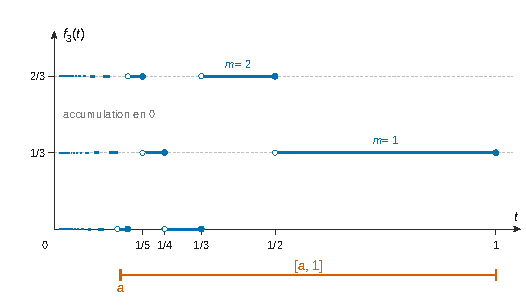
\includegraphics{figures/q18-paliers-f3.pdf}
\caption*{Figure 2 --- paliers de f₃ entre 1/(m+1) (exclu) et 1/m (inclus) :
valeurs 0, 1/3, 2/3, accumulation en 0, nombre fini de paliers sur un
segment d'origine a \textgreater{} 0 (Q18)}
\end{figure}

\begin{piege}

\(f_k\) a une infinité de discontinuités (aux points \(\frac1m\)), mais elles ne s'accumulent qu'en \(0\), borne exclue : c'est compatible avec la continuité par morceaux sur \(]0,1]\), qui s'entend sur tout segment inclus dans \(]0,1]\).

\end{piege}

\begin{methode}

Le lemme des paliers resservira en Q19, Q30, Q31 et Q33 : il vaut la peine de l'énoncer une fois pour toutes.

\end{methode}

\hypertarget{question-19}{%
\subsection{Question 19}\label{question-19}}

\begin{indication}{1}

Majorer la partie entière par son argument : on obtient une puissance de \(t\).

\end{indication}

\begin{indication}{2}

Comparer à une intégrale de Riemann en \(0\) ; préciser l'exposant critique.

\end{indication}

\hypertarget{solution-18}{%
\subsubsection{Solution}\label{solution-18}}

Par la preuve du lemme des paliers, \(t\mapsto\lfloor\frac1{kt}\rfloor\) est en escalier sur tout segment de \(]0,1]\), et son produit par \(t^{s-1}\) est continu par morceaux. Comme \(0\leqslant\lfloor u\rfloor\leqslant u\),
\equationajustee{0\leqslant\Bigl\lfloor\frac1{kt}\Bigr\rfloor t^{s-1}\leqslant\frac1kt^{s-2},}
et \(t^{s-2}=t^{-(2-s)}\) est intégrable sur \(]0,1]\) puisque \(2-s<1\). \textbf{L'intégrale converge} par comparaison de fonctions positives.

\hypertarget{question-20}{%
\subsection{Question 20}\label{question-20}}

\begin{indication}{1}

Découper \(]0,1]\) selon les intervalles où \(\lfloor\frac1t\rfloor\) est constant, en se limitant d'abord à \([\frac1{N+1},1]\).

\end{indication}

\begin{indication}{2}

Faire tendre \(N\) vers l'infini grâce à Q19, puis calculer la somme partielle obtenue par un décalage d'indice (elle n'est pas directement télescopique).

\end{indication}

\hypertarget{solution-19}{%
\subsubsection{Solution}\label{solution-19}}

Sur \(]\frac1{j+1},\frac1j]\), \(\lfloor\frac1t\rfloor=j\). Par Chasles,
\equationajustee{\int_{1/(N+1)}^1\Bigl\lfloor\frac1t\Bigr\rfloor t^{s-1}\,\mathrm dt=\sum_{j=1}^Nj\int_{1/(j+1)}^{1/j}t^{s-1}\,\mathrm dt,}
et le membre de gauche tend vers \(F(s)\) (Q19, \(k=1\)) : la série converge, de somme \(F(s)\). Puis \(\int_{1/(j+1)}^{1/j}t^{s-1}\,\mathrm dt=\frac1s(j^{-s}-(j+1)^{-s})\) et
\equationajustee{\begin{aligned}\sum_{j=1}^Nj\bigl(j^{-s}-(j+1)^{-s}\bigr)&=\sum_{j=1}^Nj^{1-s}-\sum_{i=2}^{N+1}(i-1)i^{-s}\\&=\sum_{i=1}^{N+1}i^{-s}-(N+1)^{1-s}\\&\xrightarrow[N\to+\infty]{}\zeta(s).\end{aligned}}
Donc
\equationajustee{\boxed{\begin{aligned}F(s)&=\sum_{j=1}^{+\infty}j\int_{1/(j+1)}^{1/j}t^{s-1}\,\mathrm dt\\&=\frac{\zeta(s)}s.\end{aligned}}}

\begin{methode}

Pour intégrer une fonction en escalier à infinité de paliers sur \(]0,1]\), on applique Chasles sur un segment \([\varepsilon_N,1]\) puis on passe à la limite grâce à la convergence de l'intégrale. Aucun théorème d'interversion n'est nécessaire.

\end{methode}

\begin{piege}

Ne pas perdre le terme \(-(N+1)^{1-s}\) dans le décalage d'indice : il tend vers \(0\) parce que \(s>1\), et c'est là que sert l'hypothèse.

\end{piege}

\hypertarget{question-21}{%
\subsection{Question 21}\label{question-21}}

\begin{indication}{1}

Par linéarité (deux intégrales convergentes), il suffit de calculer \(\int_0^1\lfloor\frac1{kt}\rfloor t^{s-1}\,\mathrm dt\).

\end{indication}

\begin{indication}{2}

Déterminer les intervalles où \(\lfloor\frac1{kt}\rfloor=j\) et refaire le calcul de Q20 : un facteur \(k^{-s}\) apparaît.

\end{indication}

\hypertarget{solution-20}{%
\subsubsection{Solution}\label{solution-20}}

Les deux intégrales \(F(s)\) et \(I_k(s)=\int_0^1\lfloor\frac1{kt}\rfloor t^{s-1}\,\mathrm dt\) convergent (Q19), donc
\equationajustee{\int_0^1f_kt^{s-1}=\frac1kF(s)-I_k(s).}
L'intégrande de \(I_k\) est nul sur \(]\frac1k,1]\), et \(\lfloor\frac1{kt}\rfloor=j\) sur \(]\frac1{k(j+1)},\frac1{kj}]\). Comme en Q20,
\equationajustee{\begin{aligned}I_k(s)&=\sum_{j\geqslant1}\frac js\Bigl(\frac1{(kj)^s}-\frac1{(k(j+1))^s}\Bigr)\\&=\frac1{k^s}\cdot\frac1s\sum_{j\geqslant1}j\bigl(j^{-s}-(j+1)^{-s}\bigr)\\&=\frac{\zeta(s)}{s\,k^s}.\end{aligned}}
D'où
\equationajustee{\boxed{\int_0^1f_k(t)t^{s-1}\,\mathrm dt=\frac1s\Bigl(\frac1k-\frac1{k^s}\Bigr)\zeta(s).}}

\begin{piege}

Le changement de variable \(u=kt\) est tentant, mais le théorème du programme pour les intégrales généralisées suppose la fonction continue ; le découpage en paliers (ou un changement de variable sur chaque palier) évite la difficulté.

\end{piege}

\begin{methode}

C'est la formule pivot du sujet : \(\zeta\) apparaît en facteur, donc tout zéro de \(\zeta\) annule simultanément toutes ces intégrales. C'est exactement ce qu'exploite Q38.

\end{methode}

\hypertarget{b.ii-prolongement-de-la-fonction-zeta}{%
\subsection{\texorpdfstring{B.II --- Prolongement de la fonction \(\zeta\)}{B.II --- Prolongement de la fonction \textbackslash zeta}}\label{b.ii-prolongement-de-la-fonction-zeta}}

\hypertarget{question-22}{%
\subsection{Question 22}\label{question-22}}

\begin{indication}{1}

Dériver et étudier la monotonie de \(|h'|\).

\end{indication}

\hypertarget{solution-21}{%
\subsubsection{Solution}\label{solution-21}}

\(|h'(t)|=\frac s{t^{s+1}}\) est décroissante sur \([k,k+1]\), d'où
\equationajustee{\boxed{\max_{[k,k+1]}|h'|=\frac s{k^{s+1}}.}}

\hypertarget{question-23}{%
\subsection{Question 23}\label{question-23}}

\begin{indication}{1}

Positivité : monotonie de \(t\mapsto t^{-s}\). Majoration : inégalité des accroissements finis avec Q22.

\end{indication}

\begin{indication}{2}

Sommer les majorations et reconnaître \(\zeta(s+1)\), qui existe car \(s+1>1\) même si \(s\leqslant1\).

\end{indication}

\hypertarget{solution-22}{%
\subsubsection{Solution}\label{solution-22}}

Pour \(t\in[k,k+1]\), \(t^{-s}\leqslant k^{-s}\), donc \(w_k=\int_k^{k+1}(k^{-s}-t^{-s})\,\mathrm dt\geqslant0\). Par l'inégalité des accroissements finis et Q22,
\equationajustee{0\leqslant k^{-s}-t^{-s}\leqslant\frac s{k^{s+1}}(t-k)\leqslant\frac s{k^{s+1}},}
donc \(0\leqslant w_k\leqslant\frac s{k^{s+1}}\). La série \(\sum\frac s{k^{s+1}}=s\zeta(s+1)\) converge, d'où la convergence de \(\sum w_k\) et
\equationajustee{\boxed{0\leqslant G(s)\leqslant s\,\zeta(s+1).}}

\begin{figure}[H]
\centering
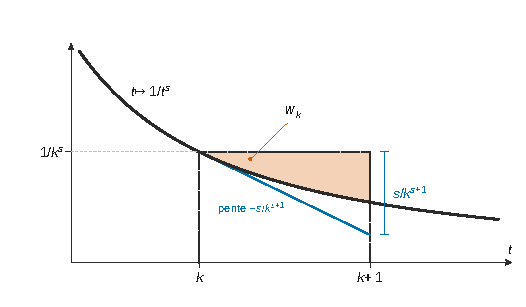
\includegraphics{figures/q23-comparaison-serie-integrale.pdf}
\caption*{Figure 3 --- w\_k est l'aire entre le palier de hauteur 1/kˢ et la
courbe t ↦ 1/tˢ, de k à k+1 ; l'écart vertical est majoré par s/kˢ⁺¹
(Q23)}
\end{figure}

\begin{piege}

Majorer \(w_k\) par \(k^{-s}\) donnerait une série divergente pour \(s\leqslant1\), précisément le cas qui intéresse le prolongement.

\end{piege}

\hypertarget{question-24}{%
\subsection{Question 24}\label{question-24}}

\begin{indication}{1}

Calculer les sommes partielles de \(G(s)\) par Chasles : on obtient une somme partielle de \(\zeta\) moins une intégrale explicite.

\end{indication}

\begin{indication}{2}

Pour le \(O(1)\), borner \(G\) sur un intervalle \(]1,2]\) en utilisant la monotonie de \(\zeta\).

\end{indication}

\hypertarget{solution-23}{%
\subsubsection{Solution}\label{solution-23}}

Pour \(s>1\),
\equationajustee{\begin{aligned}\sum_{k=1}^Nw_k&=\sum_{k=1}^Nk^{-s}-\int_1^{N+1}t^{-s}\,\mathrm dt\\&=\sum_{k=1}^Nk^{-s}-\frac{1-(N+1)^{1-s}}{s-1}\\&\xrightarrow[N\to+\infty]{}\zeta(s)-\frac1{s-1},\end{aligned}}
d'où
\equationajustee{\boxed{\zeta(s)-G(s)=\frac1{s-1}.}}
Pour \(s\in\,]1,2]\), comme \(\zeta\) est décroissante,
\equationajustee{0\leqslant G(s)\leqslant s\zeta(s+1)\leqslant2\zeta(2),}
donc \(G(s)=O(1)\) et
\equationajustee{\boxed{\zeta(s)=\frac1{s-1}+O(1)\quad(s\to1^+).}}

\begin{methode}

Comparaison série-intégrale : la différence \(\sum k^{-s}-\int t^{-s}\) reste contrôlée même quand chacun des deux termes diverge. C'est ce qui permet de \emph{définir} \(\zeta(s)=\frac1{s-1}+G(s)\) pour \(0<\operatorname{Re}(s)\leqslant1\), \(s\neq1\).

\end{methode}

\hypertarget{b.iii-intuxe9grale-des-fonctions-f_k}{%
\subsection{\texorpdfstring{B.III --- Intégrale des fonctions \(f_k\)}{B.III --- Intégrale des fonctions f\_k}}\label{b.iii-intuxe9grale-des-fonctions-f_k}}

\hypertarget{question-25}{%
\subsection{Question 25}\label{question-25}}

\begin{indication}{1}

Pour \(s>1\) et \(t\in\,]0,1]\), comparer \(t^{s-1}\) à \(1\).

\end{indication}

\begin{indication}{2}

Majorer l'écart entre les deux intégrales en utilisant la borne de Q16 ; ou appliquer la convergence dominée avec une domination indépendante de \(s\).

\end{indication}

\hypertarget{solution-24}{%
\subsubsection{Solution}\label{solution-24}}

Pour \(s>1\), \(0<t^{s-1}\leqslant1\) sur \(]0,1]\), donc par Q16
\equationajustee{\begin{aligned}\Bigl|\int_0^1f_k(t)\bigl(t^{s-1}-1\bigr)\mathrm dt\Bigr|&\leqslant\frac{k-1}k\int_0^1(1-t^{s-1})\,\mathrm dt\\&=\frac{k-1}k\Bigl(1-\frac1s\Bigr)\\&\xrightarrow[s\to1^+]{}0.\end{aligned}}
Donc
\equationajustee{\boxed{\int_0^1f_k(t)t^{s-1}\,\mathrm dt\xrightarrow[s\to1^+]{}\int_0^1f_k(t)\,\mathrm dt.}}
Le théorème de convergence dominée à paramètre réel, avec la domination \(|f_k(t)t^{s-1}|\leqslant\frac{k-1}k\) indépendante de \(s\), donne le même résultat.

\hypertarget{question-26}{%
\subsection{Question 26}\label{question-26}}

\begin{indication}{1}

Faire tendre \(s\) vers \(1^+\) dans Q21 : forme indéterminée \(0\times\infty\).

\end{indication}

\begin{indication}{2}

Remplacer \(\zeta(s)\) par \(\frac1{s-1}+G(s)\) (Q24) et traiter séparément les deux termes ; pour le premier, faire apparaître un taux d'accroissement de l'exponentielle.

\end{indication}

\hypertarget{solution-25}{%
\subsubsection{Solution}\label{solution-25}}

Pour \(s\in\,]1,2]\),
\equationajustee{\int_0^1f_kt^{s-1}=\frac1s\cdot\frac{\frac1k-k^{-s}}{s-1}+\frac1s\Bigl(\frac1k-k^{-s}\Bigr)G(s).}
Avec \(u=(s-1)\ln k\),
\equationajustee{\frac{\frac1k-k^{-s}}{s-1}=\frac{\ln k}k\cdot\frac{1-e^{-u}}u\xrightarrow[s\to1^+]{}\frac{\ln k}k.}
Le second terme tend vers \(0\) (\(G\) bornée, Q24). Par Q25 et unicité de la limite :
\equationajustee{\boxed{\int_0^1f_k(t)\,\mathrm dt=\frac{\ln k}k.}}
Contrôle : \(\int_0^1f_2=\frac{\ln2}2\approx0{,}347\in[0,\frac12]\), cohérent avec Q16.

\begin{piege}

Écrire « \(\zeta(s)\sim\frac1{s-1}\) donc le produit tend vers \(\frac{\ln k}k\) » est acceptable à condition de montrer que l'autre facteur divisé par \(s-1\) a une limite finie ; la décomposition par \(G\) évite toute ambiguïté.

\end{piege}

\hypertarget{partie-c-uxe9tude-alguxe9brique-et-guxe9omuxe9trique}{%
\section{Partie C --- Étude algébrique et géométrique}\label{partie-c-uxe9tude-alguxe9brique-et-guxe9omuxe9trique}}

On construit le cadre préhilbertien : l'espace \(L^2\) des fonctions continues par morceaux de carré intégrable sur \(]0,1]\), puis la forme \((f|g)=\int_0^1fg\).

Cette forme n'est que positive sur \(L^2\), mais elle est définie sur \(F=\operatorname{Vect}(\mathbf 1,f_2,f_3,\dots)\). Viennent ensuite la liberté de \((f_k)\), puis la distance \(d_n\).

\hypertarget{c.i-une-forme-bilinuxe9aire-symuxe9trique-positive}{%
\subsection{C.I --- Une forme bilinéaire symétrique positive}\label{c.i-une-forme-bilinuxe9aire-symuxe9trique-positive}}

\hypertarget{question-27}{%
\subsection{Question 27}\label{question-27}}

\begin{indication}{1}

Une affirmation vraie se démontre, une affirmation fausse se réfute par un contre-exemple dont on vérifie les deux propriétés.

\end{indication}

\begin{indication}{2}

Penser aux fonctions \(t\mapsto t^{-\alpha}\) : pour quels \(\alpha\) sont-elles intégrables, de carré intégrable sur \(]0,1]\) ?

\end{indication}

\hypertarget{solution-26}{%
\subsubsection{Solution}\label{solution-26}}

\textbf{a) Vraie} : si \(|f|\leqslant M\), \(f^2\leqslant M^2\), intégrable sur l'intervalle borné \(]0,1]\).

\textbf{b) Fausse} : \(t\mapsto\frac1t\in E\) mais \(\int_\varepsilon^1t^{-2}\,\mathrm dt=\frac1\varepsilon-1\to+\infty\).

\textbf{c) Fausse} : \(t\mapsto t^{-1/2}\) est intégrable (\(\int_0^1t^{-1/2}=2\)) mais son carré \(\frac1t\) ne l'est pas.

\begin{methode}

Sur \(]0,1]\), \(t^{-\alpha}\) est intégrable si et seulement si \(\alpha<1\), de carré intégrable si et seulement si \(\alpha<\frac12\) : les contre-exemples se prennent dans la bande \(\frac12\leqslant\alpha<1\).

\end{methode}

\hypertarget{question-28}{%
\subsection{Question 28}\label{question-28}}

\begin{indication}{1}

Développer \((|f|-|g|)^2\geqslant0\).

\end{indication}

\begin{indication}{2}

Pour la stabilité, développer \((f+\lambda g)^2\) : les trois intégrales qui apparaissent convergent.

\end{indication}

\hypertarget{solution-27}{%
\subsubsection{Solution}\label{solution-27}}

\((|f|-|g|)^2\geqslant0\) donne \(|fg|\leqslant\frac12(f^2+g^2)\), majorant intégrable si \(f,g\in L^2\) : \textbf{\(\int_0^1fg\) converge absolument.}

Ensuite \(0\in L^2\). Pour \(f,g\in L^2\) et \(\lambda\in\mathbb R\), la fonction
\equationajustee{(f+\lambda g)^2=f^2+2\lambda fg+\lambda^2g^2}
a une intégrale convergente : \(f+\lambda g\in L^2\). \textbf{\(L^2\) est un sous-espace vectoriel de \(E\).}

\begin{piege}

Invoquer Cauchy-Schwarz ici serait circulaire : la forme \((\cdot|\cdot)\) n'est pas encore définie. L'ordre logique est : convergence de \(\int fg\), puis stabilité.

\end{piege}

\hypertarget{question-29}{%
\subsection{Question 29}\label{question-29}}

\begin{indication}{1}

Bilinéarité, symétrie et positivité découlent des propriétés de l'intégrale.

\end{indication}

\begin{indication}{2}

Pour le contre-exemple, chercher une fonction continue par morceaux, non nulle, mais nulle sauf en un point.

\end{indication}

\hypertarget{solution-28}{%
\subsubsection{Solution}\label{solution-28}}

\((f|g)\) est défini par Q28 ; la linéarité de l'intégrale donne la linéarité à gauche, la symétrie est évidente (d'où la linéarité à droite), et \((f|f)=\int_0^1f^2\geqslant0\). \textbf{C'est une forme bilinéaire symétrique positive.}

Soit \(u\) définie par \(u(1)=1\) et \(u=0\) sur \(]0,1[\). Elle est continue par morceaux, bornée, donc dans \(L^2\).

Elle est non nulle, et \((u|u)=0\). \textbf{Ce n'est pas un produit scalaire sur \(L^2\).}

\begin{piege}

Le contre-exemple doit être continu par morceaux : l'indicatrice de \(\mathbb Q\) ne convient pas.

\end{piege}

\hypertarget{c.ii-un-espace-pruxe9hilbertien-ruxe9el}{%
\subsection{C.II --- Un espace préhilbertien réel}\label{c.ii-un-espace-pruxe9hilbertien-ruxe9el}}

\hypertarget{question-30}{%
\subsection{Question 30}\label{question-30}}

\begin{indication}{1}

Que valent les deux parties entières pour \(t\in\,]\frac12,1]\) et \(k\geqslant2\) ?

\end{indication}

\hypertarget{solution-29}{%
\subsubsection{Solution}\label{solution-29}}

Pour \(t\in\,]\frac12,1]\), \(\lfloor\frac1t\rfloor=1\) et \(0<\frac1{kt}<\frac2k\leqslant1\), donc \(\lfloor\frac1{kt}\rfloor=0\) et \(f_k(t)=\frac1k\). En évaluant la relation en un tel \(t\) :
\equationajustee{\boxed{\sum_{k=2}^n\frac{\lambda_k}k=0.}}

\begin{piege}

L'inégalité \(t>\frac12\) doit être stricte : en \(t=\frac12\), \(f_2(\frac12)=0\).

\end{piege}

\hypertarget{question-31}{%
\subsection{Question 31}\label{question-31}}

\begin{indication}{1}

Évaluer en \(t=\frac1\ell\).

\end{indication}

\begin{indication}{2}

Séparer les indices \(k>\ell\), \(k=\ell\) et \(k<\ell\) ; le terme \(k=\ell\) a une valeur remarquable.

\end{indication}

\hypertarget{solution-30}{%
\subsubsection{Solution}\label{solution-30}}

En \(t=\frac1\ell\), on a \(f_k(\frac1\ell)=\frac\ell k-\lfloor\frac\ell k\rfloor\).

Ce nombre vaut \(\frac\ell k\) si \(k>\ell\) et \(0\) si \(k=\ell\) ; il reste tel quel si \(k<\ell\).

D'où
\equationajustee{\boxed{\begin{aligned}{}&\sum_{k=\ell+1}^n\lambda_k\frac\ell k\\&\quad+\sum_{k=2}^{\ell-1}\lambda_k\Bigl(\frac\ell k-\Bigl\lfloor\frac\ell k\Bigr\rfloor\Bigr)=0.\end{aligned}}}

\begin{methode}

Évaluer une relation fonctionnelle en des points bien choisis transforme une identité entre fonctions en un système linéaire, ici triangulaire grâce à l'annulation du terme \(k=\ell\).

\end{methode}

\hypertarget{question-32}{%
\subsection{Question 32}\label{question-32}}

\begin{indication}{1}

Soustraire Q31 pour \(\ell=2\) (divisée par \(2\)) de Q30.

\end{indication}

\begin{indication}{2}

Pour la suite, formuler une récurrence portant à la fois sur l'annulation des premiers \(\lambda_k\) et sur une relation du type de Q30 commençant à l'indice \(\ell\). Ne pas oublier le dernier coefficient.

\end{indication}

\hypertarget{solution-31}{%
\subsubsection{Solution}\label{solution-31}}

Si \(n=2\), Q30 donne \(\lambda_2=0\). Sinon, Q31 pour \(\ell=2\) donne \(\sum_{k=3}^n\frac{\lambda_k}k=0\), et la différence avec Q30 donne \(\lambda_2=0\).

Récurrence : pour \(2\leqslant\ell\leqslant n\), on note \((\mathcal H_\ell)\) la propriété
\equationajustee{\begin{aligned}{}&\lambda_2=\dots=\lambda_{\ell-1}=0\\&\text{et}\ \sum_{k=\ell}^n\frac{\lambda_k}k=0.\end{aligned}}
\((\mathcal H_2)\) est Q30. Supposons \((\mathcal H_\ell)\) vraie avec \(\ell\leqslant n-1\).

Q31 au rang \(\ell\) se réduit à \(\ell\sum_{k=\ell+1}^n\frac{\lambda_k}k=0\). La différence avec \((\mathcal H_\ell)\) donne \(\lambda_\ell=0\) : \((\mathcal H_{\ell+1})\) est vraie.

\((\mathcal H_n)\) donne enfin \(\lambda_n=0\).

Tous les \(\lambda_k\) sont nuls : \textbf{la famille \((f_k)_{k\geqslant2}\) est libre} (toute sous-famille finie est incluse dans une famille \((f_2,\dots,f_n)\)).

\begin{piege}

Le cas terminal \(\lambda_n\) n'est pas couvert par Q31 (qui exige \(\ell\leqslant n-1\)) : il se lit sur la dernière relation. Et « de même pour \(\lambda_3\), etc. » ne constitue pas une preuve.

\end{piege}

\hypertarget{question-33}{%
\subsection{Question 33}\label{question-33}}

\begin{indication}{1}

Bilinéarité, symétrie et positivité sont héritées de Q29 ; il reste le caractère défini, qui échouait sur \(L^2\).

\end{indication}

\begin{indication}{2}

Qu'ont de particulier les éléments de \(F\) sur chaque intervalle \(]\frac1{m+1},\frac1m]\) ?

\end{indication}

\hypertarget{solution-32}{%
\subsubsection{Solution}\label{solution-32}}

\(\mathbf 1\) et les \(f_k\) sont bornées, donc dans \(L^2\) : \(F\subset L^2\) et \((\cdot|\cdot)\) y est bilinéaire symétrique positive.

Soit \(f=a\mathbf 1+\sum_{k=2}^n\lambda_kf_k\) avec \((f|f)=0\). Par le lemme des paliers, \(f\) vaut une constante \(c_m\) sur \(]\frac1{m+1},\frac1m]\), et
\equationajustee{\begin{aligned}0\leqslant c_m^2\Bigl(\frac1m-\frac1{m+1}\Bigr)&=\int_{1/(m+1)}^{1/m}f^2\\&\leqslant\int_0^1f^2=0,\end{aligned}}
donc \(c_m=0\) pour tout \(m\), et \(f=0\) sur \(]0,1]\). \textbf{\((\cdot|\cdot)\) est un produit scalaire sur \(F\).}

\begin{piege}

« \(\int f^2=0\) et \(f\) continue par morceaux, donc \(f=0\) » est faux : c'est exactement le contre-exemple de Q29. Il faut utiliser que les éléments de \(F\) sont constants sur des intervalles de longueur non nulle, y compris aux extrémités \(\frac1m\).

\end{piege}

\hypertarget{c.iii-distance-dun-vecteur-uxe0-des-sous-espaces}{%
\subsection{C.III --- Distance d'un vecteur à des sous-espaces}\label{c.iii-distance-dun-vecteur-uxe0-des-sous-espaces}}

\hypertarget{question-34}{%
\subsection{Question 34}\label{question-34}}

\begin{indication}{1}

Reconnaître le procédé de Gram-Schmidt ; quelles hypothèses demande-t-il ? (Q32, Q33.)

\end{indication}

\begin{indication}{2}

Pour l'unicité, raisonner par récurrence : \(e_p\) doit appartenir à \(\operatorname{Vect}(f_2,\dots,f_p)\) et être orthogonal à \(\operatorname{Vect}(f_2,\dots,f_{p-1})\) ; quelle est la dimension de cet ensemble ?

\end{indication}

\hypertarget{solution-33}{%
\subsubsection{Solution}\label{solution-33}}

\((F,(\cdot|\cdot))\) est préhilbertien (Q33) et \((f_2,\dots,f_n)\) est libre (Q32). Notons \(V_p=\operatorname{Vect}(f_2,\dots,f_p)\).

\emph{\(p=2\)} : \(e_2=\mu f_2\) avec \(|\mu|\,\|f_2\|=1\) et \(\mu\|f_2\|^2>0\), d'où l'unique choix \(e_2=\frac{f_2}{\|f_2\|}\).

\emph{Hérédité} : supposons \((e_2,\dots,e_{p-1})\) existante et unique, base orthonormée de \(V_{p-1}\). Le vecteur
\equationajustee{w=f_p-\sum_{j<p}(f_p|e_j)e_j}
est orthogonal à \(V_{p-1}\) et non nul (\(f_p\notin V_{p-1}\)).

Le vecteur \(e_p=\frac w{\|w\|}\) convient : la famille est orthonormale et \(\operatorname{Vect}(e_2,\dots,e_p)=V_{p-1}+\mathbb Rf_p=V_p\). De plus \((e_p|f_p)=\|w\|>0\), car \(f_p-w\in V_{p-1}\perp w\).

Si \(e'_p\) convient, \(e'_p\in V_p\cap V_{p-1}^\perp\). Écrivons \(e'_p=u+\alpha w\) avec \(u\in V_{p-1}\) : on a \(\|u\|^2=(e'_p|u)=0\), donc \(e'_p=\alpha w\).

Les conditions de norme et de signe imposent alors \(\alpha=\frac1{\|w\|}\).

\textbf{Il existe une unique famille orthonormale \((e_k)_{2\leqslant k\leqslant n}\) de \(F\subset L^2\) vérifiant les conditions demandées.} Par unicité, la famille obtenue pour \(n+1\) prolonge celle obtenue pour \(n\).

\begin{methode}

La condition de drapeau \(\operatorname{Vect}(e_2,\allowbreak \dots,\allowbreak e_p)=\operatorname{Vect}(f_2,\allowbreak \dots,\allowbreak f_p)\) force \(e_p\) à être colinéaire au vecteur de Gram-Schmidt ; la condition de signe choisit entre les deux vecteurs unitaires possibles.

\end{methode}

\hypertarget{question-35}{%
\subsection{Question 35}\label{question-35}}

\begin{indication}{1}

La distance à un sous-espace de dimension finie est réalisée par le projeté orthogonal, dont on connaît l'expression dans une base orthonormée.

\end{indication}

\begin{indication}{2}

Appliquer Pythagore et calculer \(\|\mathbf 1\|^2\).

\end{indication}

\hypertarget{solution-34}{%
\subsubsection{Solution}\label{solution-34}}

Soit \(G_n=\operatorname{Vect}(e_2,\allowbreak \dots,\allowbreak e_n)=\operatorname{Vect}(f_2,\allowbreak \dots,\allowbreak f_n)\) et \(\pi_n\) la projection orthogonale sur \(G_n\) : \(\pi_n(\mathbf 1)=\sum_{k=2}^n(\mathbf 1|e_k)e_k\) et \(d_n=\|\mathbf 1-\pi_n(\mathbf 1)\|\). Par Pythagore (\(\mathbf 1-\pi_n(\mathbf 1)\perp G_n\)) :
\equationajustee{\begin{aligned}1=\|\mathbf 1\|^2&=\|\pi_n(\mathbf 1)\|^2+d_n^2\\&=\sum_{k=2}^n(\mathbf 1|e_k)^2+d_n^2,\end{aligned}}
soit
\equationajustee{\boxed{d_n^2=1-\sum_{k=2}^n(\mathbf 1|e_k)^2.}}

\begin{figure}[H]
\centering
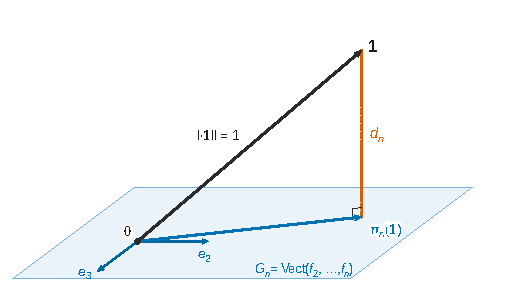
\includegraphics{figures/q35-projection-orthogonale.pdf}
\caption*{Figure 4 --- dₙ est la longueur de la composante de 𝟏 orthogonale à Gₙ ;
Pythagore donne 1 = ‖πₙ(𝟏)‖² + dₙ² (Q35)}
\end{figure}

\hypertarget{question-36}{%
\subsection{Question 36}\label{question-36}}

\begin{indication}{1}

Comparer \(G_n\) et \(G_{n+1}\), ou lire la monotonie sur Q35.

\end{indication}

\hypertarget{solution-35}{%
\subsubsection{Solution}\label{solution-35}}

\(G_n\subset G_{n+1}\), donc \(d_{n+1}=\inf_{g\in G_{n+1}}\|\mathbf 1-g\|\leqslant d_n\).

De façon équivalente, \(d_{n+1}^2=d_n^2-(\mathbf 1|e_{n+1})^2\) (la famille \((e_k)\) ne dépend pas de \(n\)). La suite \((d_n)\), décroissante et minorée par \(0\), \textbf{converge} par le théorème de la limite monotone.

\begin{piege}

Rien ne permet de calculer la limite : savoir si elle est nulle est précisément la question ouverte que le sujet relie à l'hypothèse de Riemann.

\end{piege}

\hypertarget{partie-d-synthuxe8se}{%
\section{Partie D --- Synthèse}\label{partie-d-synthuxe8se}}

On assemble : si \(\zeta(s)=0\), Q21 annule toutes les intégrales \(\int f_kt^{s-1}\) ; Cauchy-Schwarz relie alors \(\int t^{s-1}=\frac1s\) à \(d_n\), ce qui donne \(d_n^2|s|^2\geqslant2\operatorname{Re}(s)-1\), incompatible avec \(d_n\to0\).

\hypertarget{question-37}{%
\subsection{Question 37}\label{question-37}}

\begin{indication}{1}

Appliquer l'inégalité admise à deux fonctions bien choisies ; tout le travail est de vérifier ses hypothèses.

\end{indication}

\begin{indication}{2}

Pour la première fonction, utiliser Q16 et Q27 ; pour la seconde, Q4 et Q11.

\end{indication}

\hypertarget{solution-36}{%
\subsubsection{Solution}\label{solution-36}}

Soit \(u=1-\sum_{k=2}^n\lambda_kf_k\) : elle est continue par morceaux, réelle, bornée par \(1+\sum|\lambda_k|\) (Q16), donc de carré intégrable (Q27 a).

Soit \(v:t\mapsto t^{s-1}\), continue : \(|v|^2=t^{2(x-1)}=|t^{2(s-1)}|\) est intégrable car \(x>\frac12\) (Q11).

Cauchy-Schwarz admise, avec \(|u|^2=u^2\), donne
\equationajustee{\boxed{\Bigl|\int_0^1\Bigl(1-\sum_{k=2}^n\lambda_kf_k(t)\Bigr)t^{s-1}\,\mathrm dt\Bigr|^2\leqslant\int_0^1\Bigl(1-\sum_{k=2}^n\lambda_kf_k(t)\Bigr)^2\mathrm dt\times\int_0^1|t^{2(s-1)}|\,\mathrm dt.}}

\begin{jury}

Un résultat admis par l'énoncé s'applique en vérifiant explicitement chacune de ses hypothèses ; c'est ce qui est évalué dans ce type de question.

\end{jury}

\hypertarget{question-38}{%
\subsection{Question 38}\label{question-38}}

\begin{indication}{1}

Que devient le membre de gauche de Q37 si \(\zeta(s)=0\) ? Calculer \(\int_0^1t^{s-1}\,\mathrm dt\).

\end{indication}

\begin{indication}{2}

La minoration obtenue vaut pour toute famille \((\lambda_k)\) : choisir celle qui réalise la distance \(d_n\).

\end{indication}

\begin{indication}{3}

Pour conclure, faire tendre \(n\) vers l'infini (ou relire Q14).

\end{indication}

\hypertarget{solution-37}{%
\subsubsection{Solution}\label{solution-37}}

Soit \(s\neq1\), \(x=\operatorname{Re}(s)>\frac12\), avec \(\zeta(s)=0\).

\emph{Intégrale de \(t^{s-1}\)} : \(|t^{s-1}|=t^{x-1}\) est intégrable (\(x-1>-1\)) et \(\frac{t^s}s\) est une primitive. Comme \(|\varepsilon^s|=\varepsilon^x\to0\),
\equationajustee{\begin{aligned}\int_0^1t^{s-1}\,\mathrm dt&=\lim_{\varepsilon\to0^+}\frac{1-\varepsilon^s}s\\&=\frac1s.\end{aligned}}

\emph{Intégrales des \(f_k\)} : Q21 est admise pour \(s\) complexe, \(\operatorname{Re}(s)>0\), \(s\neq1\). Ces intégrales convergent absolument car \(|f_kt^{s-1}|\leqslant t^{x-1}\), et
\equationajustee{\int_0^1f_k(t)t^{s-1}\,\mathrm dt=\frac1s\Bigl(\frac1k-k^{-s}\Bigr)\zeta(s)=0.}

\emph{Inégalité} : par linéarité, \(\int_0^1(1-\sum\lambda_kf_k)t^{s-1}\,\mathrm dt=\frac1s\) pour toute famille réelle \((\lambda_k)\), et Q37 avec Q11 donne
\equationajustee{\frac1{|s|^2}\leqslant\frac{\|\mathbf 1-\sum_{k=2}^n\lambda_kf_k\|^2}{2x-1}.}
En choisissant les \(\lambda_k\) tels que \(\sum\lambda_kf_k=\pi_n(\mathbf 1)\), la norme vaut \(d_n\) (Q35) :
\equationajustee{\boxed{d_n^2|s|^2\geqslant2\operatorname{Re}(s)-1\quad\text{pour tout }n\geqslant2.}}

\emph{Conclusion} : si \(d_n\to0\), le passage à la limite donne \(0\geqslant2\operatorname{Re}(s)-1\), soit \(\operatorname{Re}(s)\leqslant\frac12\) : contradiction.

\textbf{Si \(\lim d_n=0\), \(\zeta\) prolongée ne s'annule en aucun \(s\) de partie réelle \(>\frac12\)} (\(s=1\) est un pôle, exclu de l'étude).

\emph{Lecture géométrique (facultative).} L'inégalité encadrée signifie \(s\in\Delta_{d_n}\), c'est-à-dire \(s\notin\mathcal D_{d_n}\). On a bien \(d_n\in\,]0,1[\).

\begin{itemize}
\tightlist
\item
  Soit \(L=\operatorname{ppcm}(2,\dots,n)\). Tout élément de \(G_n\) s'annule en \(\frac1L\), car \(f_k(\frac1L)=\frac Lk-\lfloor\frac Lk\rfloor=0\). Donc \(\mathbf 1\notin G_n\) et \(d_n>0\).
\item
  On a \(d_n\leqslant d_2\). Comme \(f_2\) ne prend que les valeurs \(0\) et \(\frac12\), \(\|f_2\|^2=\frac12\int_0^1f_2=\frac{\ln2}4\) ; et \((\mathbf 1|f_2)=\frac{\ln2}2\) (Q26). Donc
  \equationajustee{d_2^2=1-\frac{(\mathbf 1|f_2)^2}{\|f_2\|^2}=1-\ln2.}
\end{itemize}

Comme \(\Delta_d\subset\Delta_{d'}\) pour \(d\leqslant d'\), si \(d_n\to0\) alors \(s\in\Delta_d\) pour tout \(d\in\,]0,1[\). Donc \(\operatorname{Re}(s)\leqslant\frac12\) par Q14.

C'est la même contradiction, lue sur les disques de la partie A, qui envahissent le demi-plan \(\operatorname{Re}(s)>\frac12\) quand \(d\to0\).

\begin{methode}

Une minoration valable pour \emph{tous} les paramètres \(\lambda_k\) passe à la borne inférieure : c'est ainsi qu'une inégalité d'analyse devient une inégalité sur une distance.

\end{methode}

\begin{piege}

Le sujet démontre une implication (« \(d_n\to0\Rightarrow\) non-annulation »), pas l'hypothèse de Riemann. Conclure que \(\zeta\) ne s'annule pas serait un contresens.

\end{piege}

\hypertarget{bilan}{%
\section{Bilan}\label{bilan}}

\textbf{Méthodes à retenir.}

\begin{itemize}
\tightlist
\item
  Convergence normale sur un intervalle contre convergence normale sur tout \([a,+\infty[\) intérieur, et conclusion locale pour la continuité (Q1--Q2).
\item
  Familles sommables : produit de familles géométriques, réindexation par une bijection, sommation par paquets pour contrôler un reste (Q6--Q7).
\item
  Passage au logarithme d'un produit \emph{fini}, inégalités \(u\leqslant-\ln(1-u)\) et \(\ln(1+u)\leqslant u\) (Q8--Q9).
\item
  Manipulation des parties entières : encadrer par des entiers, puis exploiter qu'une inégalité stricte entre entiers fait gagner \(1\) (Q16, Q18).
\item
  Intégrale d'une fonction en escalier à infinité de paliers : Chasles sur \([\varepsilon,1]\), puis limite (Q20--Q21).
\item
  Comparaison série-intégrale par les accroissements finis, et prolongement d'une fonction en isolant son pôle (Q23--Q24).
\item
  Lever une forme \(0\times\infty\) en séparant le pôle d'un reste borné (Q26).
\item
  Caractère défini d'une forme intégrale : il échoue en général pour les fonctions continues par morceaux, et doit être justifié par la structure particulière du sous-espace (Q29, Q33).
\item
  Gram-Schmidt avec unicité, projection orthogonale et Pythagore (Q34--Q35).
\end{itemize}

\textbf{Prérequis à revoir.} Théorèmes sur les séries de fonctions ; familles sommables ; critères d'intégrabilité de Riemann en \(0\) ; espaces préhilbertiens (projection sur un sous-espace de dimension finie) ; module d'une puissance complexe.

\textbf{Questions classiques transposables.} Le produit eulérien et la non-annulation de \(\zeta\) sur \(\operatorname{Re}(s)>1\).

La formule \(\zeta(s)=\frac1{s-1}+O(1)\) en \(1^+\) ; les contre-exemples \(t^{-\alpha}\) sur \(]0,1]\) ; la distance à un sous-espace via Gram-Schmidt et la décroissance de \(d_n\) (inégalité de Bessel) ; l'usage de Cauchy-Schwarz pour transformer une identité intégrale en minoration de distance.

\end{document}
